\documentclass[a5paper,9pt,twoside]{extarticle} %,draft
\usepackage[top=14mm, bottom=14mm, inner=18mm, outer=10mm, footskip=5mm, nomarginpar]{geometry}
\setlength{\topskip}{0pt}
\setlength{\footskip}{8mm}

%%% Кодировка и локализация %%%
\usepackage[utf8]{inputenc} % кодовая страница документа
\usepackage[T2A]{fontenc} % внутренняя кодировка  TeX
\usepackage[english,russian]{babel} % локализация и переносы


%%% Гипперссылки и pdf %%%
\usepackage{cmap} % русский поиск в pdf
\usepackage[pagebackref]{hyperref} % гиперссылки
% для pagebackref после каждого bibitem нужна пустая строка или \par
\hypersetup{
    unicode, % корректная работа ссылок с кириллицей
    psdextra, % частично корректная работа ссылок с формулами (не все, ещё есть проблемы с math shift, subscript и superscript)
    pdftitle={Деформации фрактальных кубов}, % название документа
    pdfsubject={Диссертация аспиранта}, % тема документа
    pdfauthor={Дроздов Дмитрий Алексеевич}, % авторы документа
    pdfkeywords={Фрактальный квадрат, фрактальный куб, самоподоное множество}, % список ключевых слов,
    colorlinks, % текст гиперссылки будет выделяться цветом, а рамки не будет
    linkcolor=red, % цвет текста ссылок на мишени внутри документа
    pagecolor=red, % цвет текста ссылок на страницы
    filecolor=cyan, % цвет текста ссылок на локальные PDF файлы
    citecolor=blue, % цвет библиографических ссылок команды \cite
    urlcolor=blue, % цвет текста ссылок на ресурсы с URL
    % draft, % отключить все гипертекстовые опции
}


%%% Пакеты для формул %%%
\usepackage{amsmath} % удобная вёрстка многострочных формул, масштабирующийся текст в формулах, формулы в рамках и др.
\usepackage{amssymb} % несколько сотен дополнительных математических символов
\usepackage{amsthm} % окружения «теорема», «лемма» и т. п.
\usepackage{amsfonts} % Ажурный \mathbb{} и готический \mathfrak{} шрифты
\usepackage{mathrsfs} % Mathematical Script letters (шрифт Эйлера) \mathscr{}
\usepackage{euscript} % Шрифт Евклида \EuScript{}
% каллиграфический шрифт \mathcal{} не требует пакета
\usepackage{enumitem}
\usepackage{bm}
\usepackage{multicol}
% \usepackage{cite}     % оптимизирует списки цитирования
\usepackage{lastpage}

%%% Графика, изображения и цвета %%%
\usepackage[usenames]{color} % позволяет задавать цвет текста и фона, как отдельного блока, так и всего документа
\usepackage{graphicx} % Работа с графикой \includegraphics{}
\usepackage{float} % Фиксация плавабщих боксов [H]
\graphicspath{
    {./images/}, 
    {./images/img1/}, 
    {./images/img2/}, 
    {./images/img3/},
    {./images/img4/}, 
    {./images/tikz1/}, 
    {./images/tikz2/}, 
    {./images/tikz3/},
    {./images/tree/}
    }
% Вставка tikz-картинок с помощью \includestandalone[width=\textwidth]{images/tikz1/name.tex}
% requires -shell-escape
% \usepackage[mode=buildnew]{standalone} 
% \usepackage{tikz}
%     \usetikzlibrary{decorations.markings}
%     \usetikzlibrary{arrows}
%     \usetikzlibrary{arrows.meta}
%     \usetikzlibrary{cd}
%     \usetikzlibrary{calc}


%\usepackage[parentracker=true,
%             backend=biber,
%             hyperref=false,
%             bibencoding=utf8,
%             style=numeric-comp,
%             language=auto,
%             autolang=other,
%             citestyle=gost-numeric,
%             defernumbers=true,
%             bibstyle=gost-numeric,
%             sorting=ntvy,
%             ]{biblatex}
%\addbibresource{dissbib.bib}



%%% Русская традиция начертания математических знаков
\renewcommand{\le}  {\ensuremath{\leqslant}}
\renewcommand{\leq} {\ensuremath{\leqslant}}
\renewcommand{\ge}  {\ensuremath{\geqslant}}
\renewcommand{\geq} {\ensuremath{\geqslant}}
\renewcommand{\emptyset}{\varnothing}

%%% Русская традиция начертания математических функций (на случай копирования из зарубежных источников)
\renewcommand{\tan}{\operatorname{tg}}
\renewcommand{\cot}{\operatorname{ctg}}
\renewcommand{\csc}{\operatorname{cosec}}

%%% Русская традиция начертания греческих букв (греческие буквы вертикальные, через пакет upgreek)
% \usepackage{upgreek} % прямые греческие ради русской традиции
% \renewcommand{\epsilon}{\ensuremath{\upvarepsilon}}   %  русская традиция записи
% \renewcommand{\phi}{\ensuremath{\upvarphi}}
% %\renewcommand{\kappa}{\ensuremath{\varkappa}}
% \renewcommand{\alpha}{\upalpha}
% \renewcommand{\beta}{\upbeta}
% \renewcommand{\gamma}{\upgamma}
% \renewcommand{\delta}{\updelta}
% \renewcommand{\varepsilon}{\upvarepsilon}
% \renewcommand{\zeta}{\upzeta}
% \renewcommand{\eta}{\upeta}
% \renewcommand{\theta}{\uptheta}
% \renewcommand{\vartheta}{\upvartheta}
% \renewcommand{\iota}{\upiota}
% \renewcommand{\kappa}{\upkappa}
% \renewcommand{\lambda}{\uplambda}
% \renewcommand{\mu}{\upmu}
% \renewcommand{\nu}{\upnu}
% \renewcommand{\xi}{\upxi}
% \renewcommand{\pi}{\uppi}
% \renewcommand{\varpi}{\upvarpi}
% \renewcommand{\rho}{\uprho}
% %\renewcommand{\varrho}{\upvarrho}
% \renewcommand{\sigma}{\upsigma}
% %\renewcommand{\varsigma}{\upvarsigma}
% \renewcommand{\tau}{\uptau}
% \renewcommand{\upsilon}{\upupsilon}
% \renewcommand{\varphi}{\upvarphi}
% \renewcommand{\chi}{\upchi}
% \renewcommand{\psi}{\uppsi}
% \renewcommand{\omega}{\upomega}



\newcommand {\rr}  {\mathbb{R}}
\newcommand {\nn}  {\mathbb{N}}
\newcommand {\zz}  {\mathbb{Z}}
\newcommand {\bbc} {\mathbb{C}}
% \newcommand {\rd}  {\mathbb{R}^d}
% \newcommand {\rpo} {\mathbb{R}_+^1}

\newcommand {\al} {\alpha}
\newcommand {\be} {\beta}
\newcommand {\da} {\delta}
\newcommand {\Da} {\Delta}
\newcommand {\Dl} {\Delta}
\newcommand {\ga} {\gamma}
\newcommand {\Ga} {\Gamma}
\newcommand {\la} {\lambda}
\newcommand {\La} {\Lambda}
\newcommand {\om} {\omega}
\newcommand {\Om} {\Omega}
\newcommand {\sa} {\sigma}
\newcommand {\Sa} {\Sigma}
\newcommand {\te} {\theta}
\newcommand {\fy} {\varphi}
\newcommand {\Fy} {\varPhi}
\newcommand {\ep} {\varepsilon}
\newcommand {\ro} {\varrho}

\newcommand{\bd}{{\bm{d}}}
\newcommand{\bj}{{\bm{j}}}
\newcommand{\bi}{{\bm{i}}}
\newcommand{\bk}{{\bm{k}}}
\newcommand{\bu}{{\bm{u}}}
\newcommand{\bx}{{\bm{x}}}
\newcommand{\bl}{{\bf{l}}}
\newcommand{\bma}{{\bm{\alpha}}}
\newcommand{\bmb}{{\bm{\beta}}}
\newcommand{\bmg}{{\bm{\gamma}}}

\newcommand {\ra}  {\rightarrow}
\newcommand {\IN}  {\subset}
\newcommand {\NI}  {\supset}
\newcommand {\mmm} {\setminus}
\newcommand {\8}   {\infty}
\newcommand {\io}  {I^\infty}
\newcommand {\ia}  {I^*}
\newcommand {\0}   {\varnothing}
\newcommand {\dd}  {\partial}
\newcommand {\pr}  {\mathrm{pr}}
% \renewcommand{\span}{\mathrm{span}}


\newcommand {\eA} {{\EuScript A}}
\newcommand {\eJ} {{\EuScript J}}
\newcommand {\eC} {{\EuScript C}}
\newcommand {\eU} {{\EuScript U}}
\newcommand {\eP} {{\EuScript P}}
\newcommand {\eS} {{\EuScript S}}
\newcommand {\eW} {{\EuScript W}}
\newcommand {\eZ} {{\EuScript Z}}
\newcommand {\eK} {{\EuScript K}}
\newcommand {\hT} {{\hat T}}
\newcommand {\wP} {{\widetilde P}}
\newcommand {\eV} {{\mathcal V}}

\def \diam {\mathop{\rm diam} \nolimits}
\def \sup  {\mathop{\rm sup}  \nolimits}
\def \fix  {\mathop{\rm fix}  \nolimits}
\def \Lip  {\mathop{\rm Lip}  \nolimits}
\def \min  {\mathop{\rm min}  \nolimits}
\def \Ln   {\mathop{\rm Ln}   \nolimits}
\def \Id   {\mathop{\rm Id}   \nolimits}

\newcommand{\red}{\textcolor{red}}

\addto\captionsrussian{\def\refname{Публикации автора по теме диссертации}}

\begin{document}

\thispagestyle{empty}

\noindent\hfill\large{На правах рукописи}\\


\vspace{0pt plus1fill}
\begin{center}
\textbf {\large Дроздов Дмитрий Алексеевич}
\end{center}

\vspace{0pt plus3fill}
\begin{center}
\textbf {\Large Анализ на самоподобных множествах с конечным пересечением}

\vspace{0pt plus3fill}
{\large Специальность 1.1.1\ "---\\
<<Вещественный, комплексный и функциональный анализ>>}


\vspace{0pt plus1.5fill}
\Large{Автореферат}\par
\large{диссертации на соискание учёной степени\par кандидата физико-математических наук}
\end{center}

\vspace{0pt plus4fill}
{\centering Новосибирск~--- 2024\par}

% оборотная сторона обложки
\newpage
\thispagestyle{empty}
\noindent Работа выполнена в {Федеральном государственном бюджетном учреждение науки
Институт математики им. С. Л. Соболева Сибирского отделения Российской академии наук}.

\vspace{0.008\paperheight plus1fill}
\noindent%
\begin{tabular}{p{0.4\textwidth} p{0.56\textwidth}}
Научный руководитель: & \textbf{Тетенов Андрей Викторович,}\par
д. ф.-м. н., доцент,\par
Институт математики им. С. Л. Соболева Сибирского отделения Российской академии наук, %\par
ведущий научный сотрудник лаборатории теории функций

\vspace{0.013\paperheight}\\
Официальные оппоненты: &
{%
\textbf{Селезнёв Вадим Александрович,}\par
д. ф.-м. н., профессор,\par
Новосибирский государственный технический университет, %\par
заведующий кафедры инженерной математики\par
\vspace{0.01\paperheight}
\textbf{Махрова Елена Николаевна,}\par
к. ф.-м. н.,\par
Институт информационных технологий, математики и механики ННГУ им. Лобачевского, %\par
научный сотрудник и доцент кафедры дифференциальных уравнений, математического и численного анализа

}%
\vspace{0.013\paperheight} \\
Ведущая организация: &
Федеральное государственное автономное образовательное учреждение высшего образования «Сибирский федеральный университет»
\end{tabular}
\vspace{0.008\paperheight plus1fill}

\noindent Защита состоится 16.12.2024 г. в 16:00 на заседании диссертационного совета 24.1.074.01 при Федеральном государственном бюджетном учреждение науки
Институт математики им. С. Л. Соболева Сибирского отделения Российской академии наук~по адресу: 630090, г. Новосибирск, просп. академика Коптюга, д. 4.

\vspace{0.008\paperheight plus1fill}
\noindent С диссертацией можно ознакомиться в библиотеке ИМ СО РАН и на сайте \texttt{https://math.nsc.ru/dis-council/dissert}.

%\vspace{0.008\paperheight plus1fill}
%\noindent Отзывы на автореферат в двух экземплярах, заверенные печатью учреждения, просьба направлять по адресу: defenseCouncilAddress, учёному секретарю диссертационного совета~defenseCouncilNumber.

\vspace{0.008\paperheight plus1fill}
\noindent{Автореферат разослан $\underline{\hspace{0.5cm}}.\underline{\hspace{0.5cm}}.2024$ года.}

%\noindent Телефон для справок: defenseCouncilPhone.

\vspace{0.008\paperheight plus1fill}
\noindent
Учёный секретарь\\
диссертационного совета\\
24.1.074.01,\\
д. ф.-м. н. \hfill Подвигин Иван Викторович

%\mainmatter* % Нумерация страниц не изменится, но начнётся с новой страницы
\newpage

\section{История вопроса и основные направления}

Диссертация посвящена актуальным вопросам современного анализа, лежащим на стыке геометрической теории меры, фрактальной геометрии, теории графов и теории функции действительного переменного.
В диссертации исследуются самоподобные множества на плоскости и в пространстве, самоподобные дендриты и фрактальные $k$-кубы.

\subsection{Самоподобные множества}

Геометрическая теория множеств целой и дробной размерности развивается уже более века, при этом множества дробной размерности встречаются и во многих других разделах математики, таких как теория чисел и нелинейные дифференциальные уравнения.
Начало систематическому изучению таких множеств было положено работой\footnote{{\bf Mandelbrot B.}, Les objets fractals: forme hasard et dimension // Paris. Flammarion. 1975.} Б. Мандельброта 1975 года.
В этой работе такие множества были применены для описания природных явлений, а также впервые введён термин <<фрактал>>.
Термин <<фрактал>> происходит от латинских fractus (дробный) и frangere (ломать), которыми и описывается суть фрактала как нерегулярного и <<изломанного>> множества.

Мандельброт дал первое определение фрактала как множества, размерность Хаусдорфа которого превосходит топологическую, но он сам признал его неполным.
На практике строго определить фрактал не так просто.
К.~Фальконер\footnote{{\bf Falconer K. J.}, Fractal geometry: mathematical foundations and applications / K. J. Falconer. --- 3rd ed. --- New York: J.~Wiley and Sons., 2014. --- 398 p.} даёт несколько признаков, которым могут удовлетворять фракталы.
Для того, чтобы можно было назвать объект $A$ фракталом, он должен характеризоваться какими-либо из свойств, перечисленных ниже.

\begin{enumerate}
\item $A$ имеет тонкую структуру, т. е. содержит сложные структурные элементы на любых масштабах;
\item $A$ слишком неоднородно, чтобы описываться на традиционном геометрическом языке;
\item $A$ самоподобно в том или ином смысле, т. е. имеет повторяющуюся структуру в разных масштабах;
%Возможно, самоподобие приблизительное или статистическое.
\item <<Фрактальная>> размерность (например, размерность Хаусдорфа или клеточная размерность) множества $A$ превышает его топологическую размерность и зачастую является не натуральным числом;
\item $A$ можно построить через рекурсивные или итеративные схемы (что позволяет моделировать фракталы на компьютерах).
\end{enumerate}


Важным разделом фрактальной геометрии является теория самоподобных множеств.
На протяжении всей работы мы будем рассматривать именно самоподобные множества.
Понятие самоподобия упоминается довольно давно, так, например, в 1904 году Хельге фон Кох строит непрерывную кривую, не имеющую касательной ни в одной из своих точек, а в 1905 году Чезаро указывает на её самоподобие.
Из более поздних примеров самоподобных множеств можно указать на П. Леви, который в 1939 году описал самоподобные кривые, состоящие из $n$ копий одинакового размера.

Дж. Хатчинсон в 1981 г.\footnote{{\bf Hutchinson J.}, Fractals and Self-Similarity // Indiana University Mathematics Journal. 1981. Т. 30. № 5. С. 713--747.} дал строгое определение самоподобного множества $K$ как множества, являющегося объединением $\bigcup_{i=1}^mS_i(K)$ образов самого себя относительно отображений из системы сжимающих подобий $\eS=\{S_i, i=1,\ldots,m\}$.
Такое $K$ также будем называть аттрактором системы $\eS$.
В этой работе он ввёл систему понятий и чёткий математический аппарат к исследованию таких множеств.
Работа Хатчинсона послужила основой для множества дальнейших исследований.

Р. Молдин и С. Вильямс\footnote{{\bf Mauldin R. D., Williams S. C.}, Hausdorff dimension in graph directed constructions // Transactions of the American Mathematical Society. 1988. Т. 309. № 2. С. 811--829.} разработали концепцию граф-ори\-ен\-ти\-ро\-ванных систем подобий, аттрактором которых является система компактов, каждый из которых может состоять не только из своих копий, но и из копий других компактов системы.

В 1996 году М. Моран\footnote{{\bf Moran M.}, Hausdorff measure of infinitely generated self-similar sets // Monatshefte für Mathematik. 1996. Т. 122. № 4. С. 387--399.} определил бесконечно-порождённые самоподобные множества и указал условия, при которых их свойства аналогичны свойствам конечнопорождённых самоподобных множеств.

В теории самоподобных множеств часто возникает вопрос о вычислении фрактальной размерности самоподобного множества.
Под фрактальной размерностью обычно подразумевают одну из нескольких размерностей: размерность Минковского (или т.н. клеточная размерность), упаковочная размерность, размерность Ассуада, размерность Хаусдорфа и некоторые другие.
Для некоторых фракталов эти размерности могут совпадать, но в общем случае они не эквивалентны.

Фрактальная размерность самоподобного множества $K=\bigcup_{i=1}^mS_i(K)$ почти всегда зависит как от коэффициентов подобия $\Lip(S_i)$ отображений системы $\eS$, так и от взаимного расположения и структуры пересечения копий самоподобного множества.
Условия отделимости систем сжимающих подобий, порождающих эти фракталы, помогают определить то, насколько сильно расположение и структура пересечений копий самоподобного множества влияют на его фрактальную размерность.
Среди условий отделимости наиболее часто применяются условие открытого множества (OSC) и слабое условие отделимости (WSP).

П.~Моран в 1946 г.\footnote{{\bf Moran P. A. P.}, Additive functions of intervals and Hausdorff measure // Mathematical Proceedings of the Cambridge Philosophical Society. 1946. Т. 42. № 1. С. 15–23.} ввёл условие открытого множества (OSC) для самоподобных множеств на прямой, а Дж.~Хатчинсон $^6$ применил введённое Мораном условие открытого множества к системам сжимающих подобий в $\rr^n$ для любого натурального $n$.

Мы говорим, что система сжимающих подобий \linebreak $\eS=\{S_1, \ldots, S_m\}$ удовлетворяет условию открытого множества, если существует открытое множество $O$ такое, что множества $\{O_i=S_i(O) | S_i\in\eS\}$ содержатся в $O$ и попарно друг с другом не пересекаются.
Если система $\eS=\{S_1,\ldots,S_m\}$ сжимающих подобий в $\rr^n$ с коэффициентами подобия $r_1, \ldots, r_m$ удовлетворяет условию открытого множества, то хаусдорфова размерность аттрактора этой системы равна его размерности подобия $s$, которая является решением уравнения Морана
$$r_1^s+\ldots+r_m^s=1.$$

Условие открытого множества справедливо далеко не всегда. Но и в случае, когда система $\eS$ удовлетворяет OSC, его проверка может быть сопряжена с определёнными трудностями.
Например, открытое множество может иметь очень сложную структуру или состоять из бесконечного числа связных компонент.
Поэтому К.~Бандт и З.~Граф в 1992 году\footnote{{\bf Bandt C., Graf S.}, Self-Similar Sets 7. A Characterization of Self-Similar Fractals with Positive Hausdorff Measure // Proceedings of the American Mathematical Society. 1992. Т. 114. № 4. С. 995--1001.} нашли алгебраический аналог для OSC и ввели алгебраическое условие, основанное на ассоциированном семействе подобий $\mathcal{F}(\eS)$.
Это условие состоит в том, что $\Id\notin\overline{\mathcal{F}(\eS)}$. Авторы показали, что оно эквивалентно тому, что для системы $\eS$ с размерностью подобия $s$, $s$-мерная мера Хаусдорфа её аттрактора положительна, то есть
$$\Id\notin\overline{\mathcal{F}(\eS)} \Leftrightarrow H^s(K)>0.$$
Более того, при выполнении этого условия пересечения копий самоподобного множества $K$ имеют нулевую меру.

Условие открытого множества можно усилить требованием, согласно которому открытое множество $O$ и аттрактор $K$ системы $\eS$ имеют непустое пересечение.
Так получается сильное условие открытого множества (SOSC).
В 1994 г. А.~Шиф\footnote{{\bf Schief~A.}, Separation properties for self-similar sets // Proc. Amer. Math. Soc. 1994. Т. 112. №.~1. С.~111--115.} показал, что все три условия --- SOSC, OSC и условие положительности меры Хаусдорфа в размерности подобия --- эквивалентны.

В 1996 году М.~Цернер\footnote{{\bf Zerner M. P. W.}, Weak separation properties for self-similar sets // Proc. Amer. Math. Soc. -- 1996. -- Т.~124, №.~11. -- С.~3529--3539.} ввёл слабое условие отделимости (WSP).
Самоподобное множество удовлетворяет WSP, если тождественное отображение $\Id$ не является предельной точкой в ассоциированном семействе подобий $\mathcal{F}(\eS)$, то есть $\Id\notin\overline{\mathcal{F}(\eS)}\mmm\mathcal{F}(\eS)$.
Для самоподобных множеств, удовлетворяющих WSP, можно модифицировать уравнение Морана так, что решение этого уравнения будет совпадать с размерностью Хаусдорфа.
Для систем сжимающих подобий, не удовлетворяющих WSP, вычисление размерности Хаусдорфа их аттракторов может быть непростой задачей.


\subsection{Дендриты}

Дендритом называют локально связный континуум, не содержащий простых замкнутых дуг.
Вообще говоря, слово <<дендрит>> является термином из общей топологии. 
Согласно обзору\footnote{{\bf Charatonik J. J., Charatonik W. J.}, Dendrites // Aportaciones Mat. Comun. 1998. Т. 22. С. 227--253.} Я. Харатоника и В. Харатоника, история исследований в этой области охватывает более чем 75 лет.

В теории самоподобных множеств с самого её начала предпринимались попытки выработать некоторые подходы к самоподобным дендритам.
В 1985 году М. Хата\footnote{{\bf Hata M.}, On the structure of self-similar sets // Japan Journal of Applied Mathematics. 1985. Т. 2. № 2. С. 381--414.
} показал, что нетривиальный самоподобный дендрит имеет бесконечное множество концевых точек.
В 1990 году К. Бандт\footnote{{\bf Bandt C., Stahnke J.}, Self-similar sets 6. Interior distance on deterministic fractals // preprint, 1990} показал, что кратчайшие дуги, соединяющие пары точек самоподобной границы в посткритически конечном самоподобном множестве, являются аттракторами граф-ориентированных систем, а множество возможных значений размерностей таких дуг конечно.
Такие дуги с минимальной размерностью и мерой называются кратчайшими дугами.
В случае самоподобных дендритов, эти результаты описывают главные дуги.

К. Бандт также рассмотрел факторизацию индексного пространства, приводящую к появлению дендритов.
Дж. Кигами в своей работе\footnote{{\bf Kigami J.}, Harmonic Calculus on Limits of Networks and Its Application to Dendrites // Journal of Functional Analysis. 1995. Т. 128. № 1. С. 48--86.} применил к дендритам методы гармонического анализа на фракталах.

В работах последней четверти ХХ века рассматривались несколько важных примеров самоподобных дендритов.
К ним можно отнести дерево Хаты, множество Вичека или пентадендрит.
Тем не менее, долгое время отсутствовали удобные геометрические методы, позволяющие целенаправленно конструировать системы сжимающих подобий, аттракторы которых являлись бы дендритами.
Позднее, в статье\footnote{{\bf Тетенов~А.~В.}, О дендритах, заданных системами полиэдров и их точках ветвления / А.~В.~Тетенов, М.~Самуэль, Д.~А.~Ваулин // Труды ИММ УРО РАН, 2017, т.23, № 4, С.~281 -- 291.} были описаны методы задания и геометрические свойства самоподобных дендритов в $\rr^d$ --- вопросы, до 2017 года ещё недостаточно освещённые в теории самоподобных фракталов.
Для этого был построен и исследован класс $P$-полиэдральных дендритов в $\rr^d$.
Такие дендриты $K$ определяются как аттракторы систем $\eS = \{S_1,\ldots, S_m\}$ сжимающих подобий в $\rr^d$, переводящих заданный полиэдр $P \IN \rr^d$ в полиэдры $P_i \IN P$, попарные пересечения которых либо пусты, либо одноточечны и при этом являются общими вершинами полиэдров $P_i $, а граф попарных пересечений системы полиэдров $P_i$ ацикличен.
Эти же авторы в работе\footnote{{\bf Samuel M., Tetenov A. V., Vaulin D. A.}, Self-similar dendrites generated by polygonal systems in the plane // Siberian Electronic Mathematical Reports. 2017. Т. 14. С. 737--751.} более подробно изучили стягиваемые $P$-полигональные системы --- двумерный частный случай $P$-полиэдральных систем и привели
примеры изоморфизмов между аттракторами двух геометрически различных полигональных систем.
Это привело к поиску более широкого класса дендритов путём ослабления условий, задающих стягиваемые $P$-полигональные системы.
Исследование такого класса дендритов является одной из целей данной работы.

Говоря о полигональных системах, нельзя не упомянуть о полигаскетах, описанных К. Бандтом и Й. Штанке в работе$^{12}$ и Р. Стритчартсом в работе\footnote{{\bf Strichartz R.}, Isoperimetric Estimates on Sierpinski Gasket Type Fractals // Transactions of the American Mathematical Society. 1999. Т. 351. № 5. С. 1705--1752.}, которые хоть и не являются дендритами, но для их построения использовались схожие геометрические методы.
Для полигаскетов ими также были описаны кратчайшие дуги, соединяющие пару точек полигаскета и имеющих минимальную размерность и меру.
Кратчайшие дуги позднее будут применены в работах$^{14\ 15}$ для построения главных дуг и главного дерева самоподобного дендрита, являющегося аттрактором полигональных систем.

Проверка того, является ли самоподобное множество дендритом, связана со структурой попарных пересечений копий этого аттрактора.
Следует начать с результатов М.~Хаты$^{11}$, который в 1985 году доказал для самоподобного множества критерий связности.
Опишем эквивалентную формулировку этого критерия.

Рассмотрим для самоподобного множества его граф пересечений, в котором вершинам графа соответствуют копии самоподобного множества, а рёбра соединяют вершины, для которых соответствующие копии имеют непустое пересечение.
М.~Хата показал, что самоподобное множество $K$ связно тогда и только тогда, когда его граф пересечений связен.
При этом, если $K$ связно, то оно локально связно и линейно связно.

В дальнейшем К. Бандт и К. Келлер (1991) показали, что если у самоподобного множества копии пересекаются не более чем по одной точке и его граф пересечений есть дерево, то это множество является дендритом. Для дендритов, в которых по одной точке пересекались более двух копий, ими была сформулирована идея двудольного графа пересечений.
Завершил доказательство этой идеи А. В. Тетенов\footnote{{\bf Tetenov A.}, Finiteness properties for self-similar continua // arXiv:2003.04202v2 [math.MG]. 2021.}, определив двудольный граф пересечений, в котором одной доле соответствуют копии аттрактора, а другой доле --- точки попарных пересечений этих копий. Ребром в графе могут соединятся только точки разных долей, если соответствующая точка пересечения лежит в соответствующей копии.
Таким образом было получено необходимое и достаточное условие того, что самоподобные множества с одноточечным пересечением являются дендритами.

Данная диссертация в значительной степени посвящена изучению самоподобных дендритов.
Во второй главе определяются обобщённые полигональные системы и даются условия, при которых аттрактор такой системы будет дендритом.
В третьей главе представлен алгоритм, выявляющий среди фрактальных кубов дендриты с одноточечным пересечением.
В четвёртой главе более рассматриваются фрактальные квадраты, являющиеся дендритами, в частности, их самоподобные границы и главные деревья.


\subsection{Фрактальные квадраты}

Рассмотрим единичный квадрат на плоскости.
Разобьём этот квадрат на $n^2$ равных квадратов с ребром $1/n$, и в этом множестве квадратов разбиения выберем какое-то непустое подмножество.
Построим систему $\eS=\{S_1,...,S_m\}$ гомотетий, переводящих единичный квадрат в выбранные квадраты. Аттрактор $K$ этой системы мы будем называть {\em фрактальным квадратом}.
Широко известными примерами фрактальных квадратов являются множество Вичека и ковёр Серпинского.

Фрактальные квадраты являются самоподобным частным случаем самоаффинных {\em ковров Бедфорда-МакМаллена}.
Последние, в свою очередь, являются двумерным аналогом самоаффинных {\em губок Серпинского}.
Самоподобную губку Серпинского называют фрактальным кубом.

В 1984 году независимо друг от друга Т. Бедфорд\footnote{{\bf Bedford T.}, Crinkly curves, Markov partitions and dimension: Phd Thesis / University of Warwick, 1984.} и К. МакМаллен\footnote{{\bf McMullen C.}, The Hausdorff dimension of general Sierpiński carpets // Nagoya Mathematical Journal. 1984. Т. 96. С. 1–9.} определили и рассмотрели класс самоаффинных множеств, которые впоследствии стали называть коврами Бедфорда-МакМаллена.
Одним из их результатов была формула для вычисления хаусдорфовой размерности таких множеств.

Как оказалось, размерность и мера ковров Бедфорда-\linebreak МакМаллена и их многомерных аналогов обладает более сложным поведением по сравнению со своими самоподобными частными случаями.
Так, Ю.~Перес\footnote{{\bf Peres Y.}, The self-affine carpets of McMullen and Bedford have infinite Hausdorff measure // Mathematical Proceedings of the Cambridge Philosophical Society. 1994. Т. 116. № 3. С. 513--526.} в 1994 году показал, что мера Хаусдорфа (в своей размерности) у ковров Бедфорда-МакМал\-ле\-на может быть не $\sigma$-конечной.
Позднее Ю.~Перес и Р. Кеньон\footnote{{\bf Kenyon R., Peres Y.}, Measures of full dimension on affine-invariant sets // Ergodic Theory and Dynamical Systems. 1996. Т. 16. № 2. С. 307--323.} вывели формулу хаусдорфовой размерности для губок Серпинского.
М. Елекес с соавторами (2009) рассматривали меры на самоаффинных губках и на пересечениях губок при смещениях.
Подробный обзор и сравнение различных фрактальных размерностей (Хаусдорфа, клеточная, упаковочная, Ассуада и др.) для губок Серпинского в 2021 году привёл Дж. Фрейзер\footnote{{\bf Fraser J. M.}, Fractal Geometry of Bedford-McMullen Carpets // Thermodynamic Formalism / под ред. M. Pollicott, S. Vaienti. : Springer International Publishing, 2021. С. 495--516.}.
Т. Зайцева и В. Протасов (2022) исследовали структуру многомерных периодических замощений.

В 2013 году К.-С. Лау, Дж. Дж. Луо и Х. Рао\footnote{{\bf Lau K.-S., Luo J. J., Rao H.}, Topological structure of fractal squares // Mathematical Proceedings of the Cambridge Philosophical Society. 2013. Т. 155. № 1. С. 73--86.} рассмотрели топологические свойства замощений плоскости фрактальными квадратами.
Л. Кристеа и Б. Штайнски выпустили цикл работ, посвящённый выделению и исследованию поддуг во фрактальных квадратах и фрактальных треугольниках.
Они выделили один класс фрактальных квадратов, являющихся дендритами, назвав их лабиринтными фракталами и изучали случайные фракталы, принадлежащие этому классу.
Дж.-Ц. Сяо (2021) строил и изучал несвязные фрактальные квадраты с конечным числом компонент, для этого он особым образом модифицировал граф пересечений.

В третьей главе данной диссертации рассматривается структура и свойства пересечения пары фрактальных $k$-кубов.
В четвёртой главе более подробно рассмотрены самоподобная граница, свойство одноточечного пересечения и главное дерево у односвязных фрактальных квадратов.


\section{Научная новизна. Теоретическая и практическая ценность.}

На защиту выносятся следующие положения.

\begin{enumerate}
\item Найдено необходимое условие, при котором аттрактор обобщённой полигональной системы является дендритом.

\item Доказано, что при достаточно малом $\delta=\delta(\eS)>0$ аттрактор любой (удовлетворяющей условию совпадения параметров) $\delta$-деформации $\eS'$ полигональной системы $\eS$ является дендритом, изоморфным аттрактору системы $\eS$.

\item Получена формула, выражающая пересечение двух фрактальных $k$-кубов в терминах их множеств единиц.
Найдены условия, при которых такое пересечение будет пустым, конечным, счётным и несчётным.
Для конечного пересечения получена оценка мощности.

\item Разработан алгоритм, позволяющий проверить, является ли фрактальный $k$-куб дендритом с одноточечным пересечением.

\item Доказано, что нетривиальные односвязные фрактальные квадраты являются дендритами со свойством одноточечного пересечения.

\item Доказано, что нетривиальные односвязные фрактальные квадраты допускают ровно семь возможных топологических типов главного дерева.
\end{enumerate}

Перечисленные результаты являются новыми.

Работа носит теоретический характер.
Её результаты и методы могут быть использованы для дальнейшего изучения самоподобных множеств, фрактальных кубов, ковров Бедфорда-МакМаллена и губок Серпинского.
Результаты работы могут быть использованы специалистами по комплексному, действительному и функциональному анализу, топологии и фрактальной геометрии.

Результаты, полученные на основе полигональных дендритов и фрактальных квадратов, могут иметь практическое применение в радиофизике, во фрактальной реконструкции сигналов и радиолокационных изображений, в материаловедении и в других областях физики, химии и биологии.


\section{Апробация результатов.}

Основные результаты диссертации опубликованы в шести изданиях \cite{DST2021, DST2022, DT2024fqd, TD2022fs, TD2023fs, VDT2020}, пять из которых \cite{DST2021, DST2022, DT2024fqd, TD2023fs, VDT2020} опубликованы в журналах, рекомендованных ВАК.
Результаты всех работ получены авторами совместно при равном вкладе и являются неделимыми.

Результаты и основные положения диссертации докладывались на семинаре <<Геометрическая теория функций>> ИМ СО РАН (руководители:
проф. А. Д. Медных, чл.-корр. РАН А. Ю. Веснин, проф. В. В. Асеев); на семинаре <<Теория графов>> ИМ СО РАН (руководители: к.т.н. Е. В. Константинова, к.ф.-м.н. А. А. Добрынин); на семинаре <<Геометрия, топология и их приложения>> ИМ СО РАН (руководитель акад. И. А. Тайманов).

Результаты диссертации были представлены на международных конференциях <<Dynamics in Siberia>> (Новосибирск, ИМ СО РАН, 2021, 2024); 
на Международной научной студенческой конференции (Новосибирск, НГУ, 2021);
на Международной школе-конференции <<Комплексный анализ и его приложения>> (Геленджик, КубГУ, 2021); 
на Международной школе-конференции <<Siberian summer conference: Current developments in Geometry>> (Новосибирск, НГУ, ИМ СО РАН, 2021); 
на Международной конференции <<AMS Fall Western Virtual Sectional Meeting>> (University of New Mexico, 2021); 
на Международной научной конференции студентов, аспирантов и молодых учёных «Ломоносов-2022» (Москва, МГУ, 2022); 
на Международной конференции <<AMS Spring Western Virtual Sectional Meeting>> (University of Denver, 2022); 
на Международной конференции <<023w: Геометрия и топология трёхмерных многообразий>> (Сочи, МЦ Сириус, 2022); 
на Международной конференции по геометрическому анализу, посвященной памяти Ю.Г. Решетняка (Новосибирск, ИМ СО РАН, 2022); 
на Второй конференции Математических центров России (Москва, МГУ, МИАН, 2022); 
на Международной конференции <<030w: Geometric and Algebraic Methods in Knot Theory>> (Сочи, МЦ Сириус, 2023);
на Школе-конференции по геометрическому анализу
(Новосибирск, НГУ, 2023);
на Международной конференции <<Дни геометрии в Новосибирске>> (Новосибирск, ИМ СО РАН, 2023).


\section{Содержание диссертации}

Перейдём к описанию структуры работы и точным формулировкам основных результатов.
Диссертация выполнена в издательской системе \LaTeX, содержит 85 страниц и состоит из введения, четырёх глав, заключения и списка литературы.
Список литературы приведён в алфавитном порядке.
Изображения построены в программе IFStile и с помощью макропакета PGF/Tikz для системы \LaTeX.\\


В \textbf{первой главе} вводятся базовые понятия теории самоподобных множеств.

\noindent{\bf Определение 1.1.}
{\em Пусть $\eS=\{S_1, S_2, \ldots, S_m\}$ --- система (иньективных) сжимающих отображений полного метрического пространства $(X, d)$.
Непустое компактное множество $K\IN X$ называется аттрактором системы $\eS$, если
$$K = \bigcup \limits_{i=1}^m S_i (K).$$
Мы также называем множество $K$ самоподобным (инвариантным) относительно системы $\eS$.}\par

На протяжении всей работы особый интерес будут представлять самоподобные множества, являющиеся дендритами.

\noindent{\bf Определение 1.6.}
{\em {\em Дендрит} --- это локально связный континуум, не содержащий простых замкнутых дуг. }\\

Простой замкнутой дугой мы называем непрерывный иньективный образ окружности.\\

{\em Самоподобной границей} аттрактора $K$ называется множество $\dd K$ всех таких точек $x\in K$, что для некоторой композиции $S_\bj=S_{j_1}\ldots S_{j_n}$ отображений системы $\eS$ образ $S_\bj(x)$ содержится в пересечении пары копий аттрактора $K$.\\

\noindent{\bf Определение 1.13.}
{\em Пусть $K$ --- самоподобный дендрит c конечной самоподобной границей $\dd K$.
Минимальный поддендрит $\hat\gamma\IN K$, содержащий $\dd K$, называется {\em главным деревом} дендрита $K$.}\\

Если в самоподобном множестве его копии попарно пересекаются не более чем по одной точке, то мы говорим, что такое множество обладает свойством одноточечного пересечения.
Первым удобным классом самоподобных дендритов с одноточечным пересечением являются аттракторы стягиваемых полигональных систем.\\

\noindent{\bf Определение 1.11.}
{\em Пусть $P\subset\mathbb{R}^2$ --- гомеоморфный диску ограниченный многоугольник, а $ \eV_P$ --- множество его вершин.
Пусть $\eS = \{S_1, \ldots, S_m\}$ -- такая система подобий в ${\mathbb{R}}^2$, что:
\begin{itemize}[nolistsep]
\item[{\bf (D1)}] для любого $i \in I$ множество $P_i = S_i (P) \subset P$;
\item[{\bf (D2)}] для любых неравных $i, j \in I$, $P_i \bigcap P_j = \eV_{P_i} \bigcap \eV_{P_j}$, а $\#(\eV_{P_i} \bigcap \eV_{P_j})\le 1$;
\item[{\bf (D3)}] $\eV_P \subset \bigcup \limits_{i \in I} S_i (\eV_P)$;
\item[{\bf (D4)}] множество $\widetilde P = \bigcup \limits_{i = 1} ^m P_i$ стягиваемо.
\end{itemize}
Такая система $\eS$, удовлетворяющая условиям {\bf D1 -- D4}, называется {\em стягиваемой $P$-полигональной системой подобий}.}\\

\noindent{\bf Теорема 1.12.}
{\em Аттрактор $K$ стягиваемой $P$-полигональной системы подобий $\eS$ является дендритом.}\\

Обнаружить самоподобные дендриты с одноточечным пересечением позволяет двудольный граф пересечений.\\

\noindent{\bf Определение 1.9.}
{\em Пусть $K=K(\eS)$ --- самоподобное множество, обладающее свойством одноточечного пересечения.
{\em Двудольный граф пересечений} $\hat\Gamma=\hat\Gamma(\eS)$ системы $\eS$ --- это двудольный граф с долями $\eK=\{K_i:\ i\in I\}$ (белые вершины) и $\eP=\{p:\ p\in K_i\cap K_j,\ i,j\in I, i\neq j\}$ (чёрные вершины), и с множеством рёбер $E=\{(K_i,p):\ p\in K_i\}$.}\\

\noindent{\bf Теорема 1.10.}
{\em Пусть $K=K(\eS)$ --- самоподобный континуум со свойством одноточечного пересечения.
Если граф пересечений $\hat\Gamma(\eS)$ системы $\eS$ является деревом, то её аттрактор $K$ --- дендрит с одноточечным пересечением.}\\



Во \textbf{второй главе} получен более широкий класс полигональных дендритов.
Для этого были ослаблены требования, накладываемые на стягиваемые полигональные системы.

\noindent{\bf Определение 2.1.}
{\em Система $\eS=\{S_1,\ldots ,S_m\} $, удовлетворяющая условиям {\bf D2- - D4} определения 1.11, называется обобщённой $P$-полигональной системой подобий.}

Основные результаты главы затрагивают те обобщённые полигональные системы, которые являются $\delta$-деформациями стягиваемых полигональных систем.

\noindent{\bf Определение 2.4.}
{\em Пусть $\da>0$. Обобщённая $P'$-полигональная система $\eS'=\{S'_1,...,S'_m\}$ называется $\da$-деформацией $P$-полигональной системы $\eS=\{S_1,...,S_m\}$, если существует биекция $f:\bigcup\limits_{k=1}^m \eV_{P_k}\to \bigcup\limits_{k=1}^m \eV_{P'_k}$ такая, что
\begin{itemize}[nolistsep]
\item[a)] $f|_{\eV_P}$ продолжается до гомеоморфизма $\tilde f: P\to P'$;
\item[b)] $|f(x)-x|<\delta$ для любого $x\in \bigcup\limits_{k=1}^m \eV_{P_k}$;
\item[c)] $f(S_k(x))=S'_k(f(x))$ для любого $k\in I$ и $x\in \eV_P$.
\end{itemize} }

Аттрактор $K$ обобщённой полигональной системы $\eS$ уже не обязан быть дендритом, поэтому для $\eS$ требуется дополнительно проверить, что равенство $S_i(K)\cap S_j(K)=P_i\cap P_j$ выполняется.
В таком случае аттрактор $K$ стягиваемой полигональной системы $\eS$ и аттрактор $K'$ её $\delta$-деформации $\eS'$ изоморфны.\\

Рассмотрим дугу $\Gamma$ с концами в точках $A,\ B$ и такое сжимающее подобие $S$, что $S(A)=A$.
Если $S(\Gamma)\IN\Gamma$, то мы говорим, что $\Gamma$ инвариантна относительно подобия $S$.

{\em Параметром инвариантной дуги $\Gamma$ относительно конца $A$} называется отношение $\lambda:=\dfrac{\alpha}{\ln\rho}$, где $\alpha=\Delta\underset{{z\in\Gamma\mmm S(\Gamma)}}{\mathrm {Arg}}(z-A)$ и $\rho=\Lip(S)$.\\

Мы будем говорить, что обобщённая полигональная система система $\eS$ удовлетворяет {\em условию совпадения параметров}, если для каждого \linebreak $x=S_i(P)\cap S_j(P)$ (при $i\neq j$) все инвариантные дуги $\gamma_i\IN S_i(K)$ и $\gamma_j\IN S_j(K)$) с концом в $x$ имеют относительно $x$ одинаковые параметры.

Основные результаты главы формулируются в следующих теоремах.\\

\noindent{\bf Теорема 2.17} (о совпадении параметров){\bf .}
{\em
Пусть аттрактор $K$ обобщённой полигональной системы $\eS$ является дендритом.
Тогда система $\eS$ удовлетворяет условию совпадения параметров.}\\

\noindent{\bf Теорема 2.23} (о малых деформациях){\bf .}
{\em Для каждой полигональной системы $\eS$ существует такое $\delta(\eS) > 0$, что для всякой её $\delta$-деформации $\eS'$, удовлетворяющей условию совпадения параметров, аттрактор системы $\eS'$ является дендритом, изоморфным аттрактору системы $\eS$.}\\


В {\bf третьей главе} рассматриваются фрактальные $k$-кубы, структура пересечения их копий, а также пересечение пары фрактальных $k$-кубов.
В конце главы описывается последовательность действий, по которым можно определить, является ли данный фрактальный куб дендритом с одноточечным пересечением.\\

\noindent{\bf Определение 3.1.}
{\em Пусть  $D=\{d_1,\ldots,d_r\},\; d_i\in\{0,1,\ldots,n-1\}^k$, где $n\ge 2$, а $1<\#D<n^k$.
{\em Фрактальным $k$-кубом порядка $n$ с множеством единиц $D$} называют компактное множество $K\IN\rr^k$, удовлетворяющее равенству
$$K=\dfrac{K+D}{n}=\bigcup_{d_i\in D}\dfrac{d_i+K}{n}.$$}

Пусть $A=\{-1,0,1\}^k$.
Каждому вектору $\bma=(\al_1,\ldots,\al_k)\in A$ соответствует единственная грань единичного $k$-куба $P=[0,1]^k$, задаваемая равенством $P_\bma=P\cap(P+\bma)$.
Такое соответствие между множеством $A$и множеством граней $k$-куба $P$ является взаимно-однозначным.
Мы будем говорить, что $\bma\sqsubseteq\bmb$ если и только если $P_\bma\supseteq P_\bmb$.\\

Пусть $K^1$ и $K^2$ --- фрактальные $k$-кубы порядка $n$ с множествами единиц $D^1$ и $D^2$.
Гранью $K_\bma^i$ фрактального $k$-куба $K^i$ называется множество $K^i\cap P_\bma$.
Для любого $\bma\in A$ символом $F_\bma$ обозначим пересечение $K^1_\bma\cap(K^2_{-\bma}+\bma)=K^1\cap(K^2+\bma)$ пары граней фрактальных $k$-кубов $K^1$ и $K^2$.
Первый результат этой главы выражает пересечение $F_\bma$ в терминах множеств $F_\bmb$ (где $\bmb\sqsupseteq\bma$) и множеств единиц $D^1$ и $D^2$.\\

\noindent{\bf Теорема 3.7.}
{\em Семейство множеств $\{F_\bma=K^1\cap(K^2+\bma)\ :\ \bma\in A\}$ удовлетворяет системе $\Sa$ уравнений
\begin{equation}
F_\bma=\bigcup\limits_{\bmb\sqsupseteq\bma}
\dfrac{F_\bmb+G_{\bma\bmb}}{n},\text{ где } G_{\bma\bmb}=D^1\cap(D^2+n\bma-\bmb).\tag{3.3}
\end{equation}}

Отношения между множествами $F_\bma$ описываются {\em структурным графом $\Ga_\Sa$} с множеством вершин $\{\bma\in A\ :\ F_\bma\neq\0\}$ и множеством рёбер $\{(\bma, \bmb)\ :\ \bma\sqsubseteq\bmb, G_{\bma\bmb}\neq\0, F_\bmb\neq\0\}$, где ребро $(\bma, \bmb)$ направлено из $\bma$ в $\bmb$ и отмечено $G_{\bma\bmb}$.

Мы пишем $\bmb\succcurlyeq\bma$, если $\Ga_\Sa$ содержит направленный путь из $\bma$ в $\bmb$, и $\bmb\succ\bma$, если при этом $\bma\neq\bmb$.
Обозначим через $\Ga_\bma$ подграф графа $\Ga_\Sa$ с множеством вершин $\{\bmb\ :\ \bmb\succcurlyeq\bma\}$.

Следующая оценка множества $F_\bma$ является вторым результатом главы.\\

\noindent{\bf Теорема 3.11.}
{\em \begin{enumerate}[nolistsep]
\item[(1)] Если $\#G_\bmb>1$ для некоторого $\bmb\succcurlyeq\bma$, то $F_\bma$ несчётно.
\item[(2a)] Если $\#G_\bmb\leq1$ для любого $\bmb\succcurlyeq\bma$, то $F_\bma$ не более чем счетно.
\item[(2b)] Если при этом $\exists\ \bmb'\succ\bmb$ такое, что $\#G_\bmb=1$ и $F_{\bmb'}\neq\0$, то $F_\bma$ счетно.
\item[(3)] Если $\#G_\bmb=1$ для всех максимальных вершин $\bmb$ в $\Gamma_\bma$, и $G_{\bma_i}=\0$ для всех остальных вершин $\bma_i$ в $\Gamma_\bma$, то $F_\bma$ конечно.
В этом случае $\#F_\bma$ не превосходит сумму произведений $\prod \limits_{j=1}^{p-1}\# G_{\bma_j\bma_{j+1}}$, взятых по всем цепочкам $\bma=\bma_1\prec\ldots\prec\bma_p=\bmb$, где $\bmb$ максимальна в $\Gamma_\bma$.
\item[(4)] Если все $\bma_i\succcurlyeq\bma$ образуют единственную цепочку $\bma=\bma_1\prec\ldots\prec\bma_p$, в которой $G_{\bma_j}=\0$ и $\# G_{\bma_j\bma_{j+1}}=1$, $\#G_{\bma_p}=1$ для всех $j\le p-1$, то $\#F_\bma=1$.
\end{enumerate} \quad}

Далее будем полагать, что $K=K^1=K^2$.
Тогда $F_\bma=K\cap(K+\bma)$.
Фрактальный $k$-куб $K$ является множеством с одноточечным пересечением, если для каждого $\bma\succ0$ множество $F_\bma$ одноточечно.

Чтобы проверить, является ли фрактальный $k$-куб $K$ дендритом с одноточечным пересечением, нужно выполнить следующие шаги.\\

\begin{enumerate}[nolistsep]

\item Найдём все множества $G_\bma, G_{\bma\bmb}$ и выпишем систему уравнений $\Sigma$.

\item Построим структурный граф $\Ga_\Sa$ и рассмотрим подграф $\Ga_0$.

\item Проверим, является ли $K$ множеством с одноточечным пересечением.
Если это не так, то $K$ --- это не дендрит с одноточечным пересечением.

\item Построим двудольный граф пересечений $\hat\Gamma$ для фрактального куба $K$, сопоставив белым вершинам векторы из $D$.
Тогда для каждого $\bma\sqsupset0$ пара белых вершин $d, d+\bma$ соединена рёбрами с общей чёрной вершиной, если $d\in G_{0\bma}$.
Теорема 3.14 и следствие 3.15 позволит обнаружить случаи, когда чёрная вершина в $\hat\Gamma$ соединена более чем с двумя белыми вершинами.

\item Проверим, является ли граф $\hat\Gamma$ деревом.
Если $\hat\Gamma$ --- дерево, то $K$ --- дендрит с одноточечным пересечением.
\end{enumerate}



В {\bf четвёртой главе} были рассмотрены главные деревья нетривиальных односвязных фрактальных квадратов.

Фрактальные квадраты являются частным случаем фрактальных $k$-кубов при $k=2$, поэтому их более глубокое изучение в значительной степени опирается на результаты предыдущей главы.

Если у самоподобного дендрита конечная самоподобная граница, то главные деревья таких дендритов имеют конечное число концов.
Тогда мы можем перечислить все топологические типы главных деревьев.
Это позволит разбить все фрактальные квадраты на конечное число классов согласно форме главного дерева.

Первый результат текущей главы заключается в следующем.\\

\noindent{\bf Предложение 4.6.}
{\em Всякий односвязный фрактальный квадрат $K$ либо совпадает с $P$, либо является дендритом.
В последнем случае $K$ со свойством одноточечного пересечения.}\\

Из этого следует, что фрактальный квадрат $K$ является дендритом тогда и только тогда, когда его двудольный граф пересечений является деревом.\\

В дальнейшем, говоря <<односвязный фрактальный квадрат>>, мы будем иметь ввиду <<нетривиальный (то есть не совпадающий с $P$) односвязный фрактальный квадрат>>.\\

Для фрактального квадрата $K$ с множеством единиц $D$ мы определим множество
$A_D=\{\bma\in A\mmm\{(0,0)\}: G_{0\bma}\neq\0,\ F_\bma\neq\0\}.$
Тогда самоподобная граница $\dd K$ фрактального квадрата $K$ есть объединение
$\dd K=\bigcup\limits_{\bma\in A_D}F_\bma.$
Если при этом $K$ --- дендрит, то для любого $\bma\in A_D$ множество $F_\bma$ одноточечно.

Следующая теорема группирует односвязные фрактальные квадраты по типам в зависимости от расположения точек их самоподобной границы.\\

\noindent{\bf Теорема 4.9.}
{\em Пусть $K$ --- односвязный фрактальный квадрат, не являющийся отрезком.
Тогда $\#\dd K\in\{3,\ 4,\ 6\}$. \\
Если $\#\dd K=4$, то $\dd K=F_\bma\cup F_{-\bma}\cup F_\bmb\cup F_{-\bmb}$, где пара $\bma,\bmb$ принимает одно из следующих значений:
\begin{itemize}[nolistsep]
\item[{\bf A.}] $\bma=(1,0)$, $ \bmb=(0,1)$;
\item[{\bf B.}] $\bma=(1,1)$, $ \bmb=(1,-1)$;
\item[{\bf C.}] $\bma\in\{(1,1),\ (1,-1)\},\bmb\in\{(1,0),\ (0,1)\}$.
\end{itemize}
Если $\#\dd K=3$ или $\#\dd K=6$, то
\begin{itemize}[nolistsep]
\item[{\bf D.}] $\dd K=F_{(1,0)}\cup F_{(-1,0)}\cup F_{(0,1)}\cup F_{(0,-1)}\cup F_\bmb\cup F_{-\bmb}$, где $\bmb\in\{(1,1),\ (1,-1)\}$.
\end{itemize}}

Зная мощность самоподобной границы односвязных фрактальных квадратов, можно перечислить все топологические типы их главных деревьев.
Поскольку $\#\dd K\leq6$, в главном дереве не может быть более 6 концов.

Пусть $K$ --- односвязный фрактальный квадрат.
Лемма 4.10 указывает для $K$ комбинации векторов, которые не могут встречаться в множестве единиц $D$.
Согласно лемме 4.11, $Ord(x,K)\leq 2$ для любой угловой точки $x$.
Теорема 4.12 указывает количество угловых точек для каждого типа самоподобной границы.
Теорема 4.13 оценивает порядок ветвления произвольной точки $x\in K$ и гласит, что $Ord(x,K)\leq 4$ для любого $x\in K$.
Согласно предложению 4.14, если $\dd K$ типу {\bf D6} и $\gamma$ --- его главное дерево, то $Ord(x,\gamma)\leq2$ для любого $x\in\dd K$ и $Ord(x,\gamma)\leq3$ для любого $x\in\ga$.
Эти свойства ограничивает перечень допустимых типов главного дерева и позволяет сформулировать последний результат главы.\\

\noindent{\bf Теорема 4.15.}
{\em Для нетривиальных односвязных фрактальных квадратов существует только $7$ топологических типов главного дерева, модели которых показаны ниже.}
\begin{figure}[H]
\centering \Large {\bf
1. 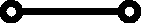
\includegraphics[width=0.15\textwidth]{mt1.pdf}
\hfill
2. 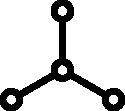
\includegraphics[width=0.15\textwidth]{mt2.pdf}
\hfill
3. 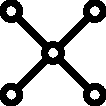
\includegraphics[width=0.13\textwidth]{mt3.pdf}
\hfill
4. 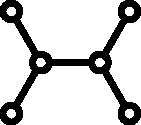
\includegraphics[width=0.15\textwidth]{mt4.pdf}\\
\bigskip
5. 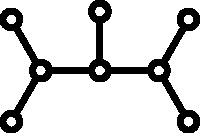
\includegraphics[width=0.23\textwidth]{mt5.pdf}
\hfill
6. 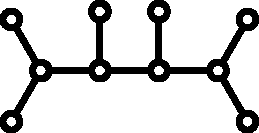
\includegraphics[width=0.3\textwidth]{mt7.pdf}
\hfill
7. 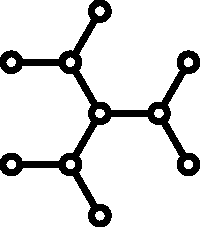
\includegraphics[width=0.22\textwidth]{mt6.pdf}}
\end{figure}

Если мы будем классифицировать односвязные фрактальные квадраты по типу главного дерева, то мы получим 7 классов.

%Если принять во внимание гипотезу о том, что во фактальном квадрате типа {\bf D6} число концов в его главном дереве $\gamma$ не меньше 4, то мы можем рассмотеть {\em тонкую классификацию}, учитывающую следующие признаки:
%\begin{itemize}[nolistsep]
% \item[1.] форма главного дерева (1 из 7 типов);
% \item[2.] тип самоподобной границы ({\bf A}, {\bf B}, {\bf C}, {\bf D3} или {\bf D6});
% \item[3.] порядки ветвления точек самоподобной границы в главном дереве.
%\end{itemize}
%Тогда мы получим 16 классов фрактальных квадратов.
%Были построены примеры фрактальных квадратов и их главных деревьев для каждого класса из тонкой классификации.






\begin{thebibliography}{9}

\bibitem{DST2021}
{\bf Drozdov D., Samuel M., Tetenov A.},
On deformation of polygonal dendrites preserving the intersection graph //
The Art of Discrete and Applied Mathematics. 2021. Т. 4. № 2. С. 1--21.

\bibitem{DST2022}
{\bf Drozdov D., Samuel M., Tetenov A.},
On $\delta$-deformations of Polygonal Dendrites //
Topological Dynamics and Topological Data Analysis. : Springer Singapore, 2021. С. 147--164.

\bibitem{DT2024fqd}
{\bf Drozdov D. A., Tetenov A. V.}, On the dendrite property of fractal cubes // Advances in the Theory of Nonlinear Analysis and Its Application. 2024. Т. 8. № 1. С. 73--80.

\bibitem{TD2022fs}
{\bf Drozdov D., Tetenov A.},
On fractal squares possessing finite intersection property //
Bulletin of National University of Uzbekistan: Mathematics and Natural Sciences. 2022. Т. 5. № 3. С. 164--181.

\bibitem{TD2023fs}
{\bf Drozdov D., Tetenov A.},
On the classification of fractal square dendrites //
Advances in the Theory of Nonlinear Analysis and Its Application. 2023. Т. 7. № 3. С. 19--96.

\bibitem{VDT2020}{\bf Ваулин Д. А., Дроздов Д. А., Тетенов А. В.},
О связных компонентах фрактальных кубов //
Труды Института математики и механики УрО РАН. 2020. Т. 26. № 2. С. 98--107.


\end{thebibliography}


%%% Выходные сведения типографии
%\newpage\thispagestyle{empty}
%
%\vspace*{0pt plus1fill}
%
%\small
%\begin{center}
%\textit{Дроздов Дмитрий Алексеевич}
%\par\medskip
%
%Анализ на самоподобных множествах с конечным пересечением
%\par\medskip
%
%Автореф. дис. на соискание учёной степени канд. физ.-мат. наук
%\par\bigskip
%
%Подписано в печать 99.99.9999.
%Заказ № 999999999999
%
%Формат 60\(\times\)90/16. Усл. печ. л. 1. Тираж 100 экз.
%%Это не совсем формат А5, но наиболее близкий, подробнее: http://ru.wikipedia.org/w/index.php?oldid=78976454
%
%Типография AAAAAAAAAAAAAAAAAAAAAA
%\end{center}
%\cleardoublepage

\end{document}